\documentclass[12pt, a4paper]{article}
\usepackage[utf8]{inputenc}
\usepackage[ngerman]{babel}
\usepackage{csquotes}
\usepackage{pdfpages}
\usepackage{graphicx}
\title{Übungsblatt 2}
\author{Thomas Samy Dafir}
\date{}

\begin{document}
	\section{18}
	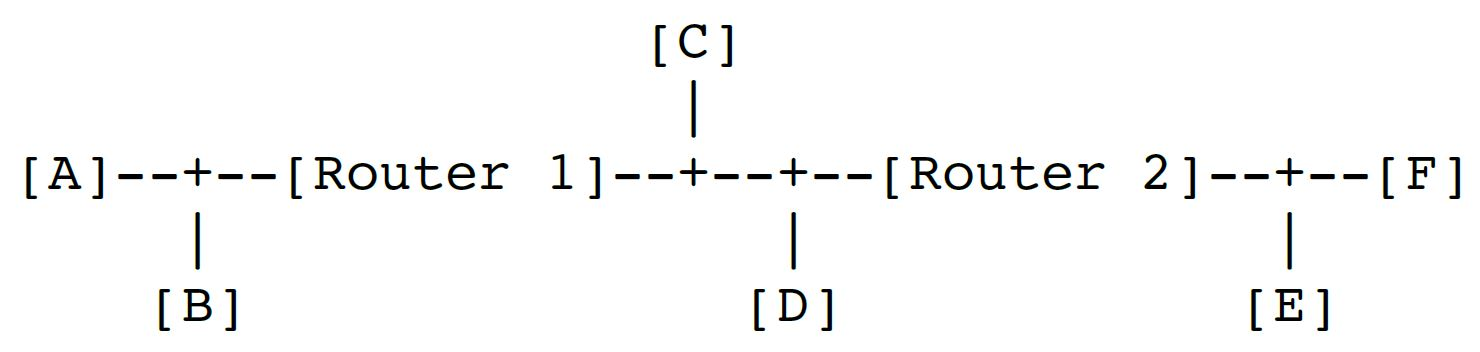
\includegraphics[width = 10cm]{18.jpg}
	\begin{itemize}
		\item A sendet als erstes eine ARP Anforderung nach B im eigenen Netzwerk. ARP fordert die MAC- oder IP-
			Adresse an.
		\item B muss sich vergewissern, dass seine eigene Adresse die Empfänger-Adresse ist. Dies trifft hier nicht zu.
		\item Die Anfrage wird über Router 1 ins nächste LAN weitergeleitet. C und D bekommen einen ARP-request.
		\item Wieder ist weder C noch D der richtige Empfänger.
		\item Die Anfrage wird über Router 2 ins nächste LAN weitergeleitet. E und F erhalten eine Anforderung.
		\item F stellt nun fest, dass er der Empfänger der von A zu sendenden Nachricht ist.
		\item F schickt ein ARP-Reply (seine IP-Adresse) an A (die Anfangsadresse) zurück.
		\item A trägt die Adresse in seine ARP Tabelle ein.
		\item A kann nun das Datagram an F übertragen.
	\end{itemize}
	
	\section{21}
	Ein Paket kann auf seinem Weg vom Sender zum Empfänger verschiedene/mehrere Netzwerke durchlaufen. Die Netzwerke sind
	jeweils durch Router verbunden. Router beinhalten eine Routing-Tabelle, die Informationen über die erreichbaren Netze.
	Die Tabelleneinträge umfassen: direkt verbundene Netze, statische, manuell festgelegte und eingetragene Routen und dynamische Routen.
	Ein Eintrag umfasst mindestens:
	\begin{itemize}
		\item Netzadresse und Subnetzmaske: Identifizieren gemeinsam das Ziel  des Eintrags
		\item next hop oder Gateway: Nächster Router an den ein Paket, dass an die angegebene Adresse gesendet werden soll
		weitergeleitet werden muss.
		\item Metrik: gibt an, wie effizient Pakete über die Angegebene Route gesendet werden können. Sind mehrere Routen
		vorhanden, wird die Route mit der geringsten Metrik ausgewählt.
	\end{itemize}
	Der Router oder Host ermittelt das Zielnetz, indem er ein logisches UND der Zieladresse und der Netzmasken in seiner Routing-Tabelle auswertet. Sind das Zielnetz und der Eintrag in der Routing-Tabelle gleich, wird das IP-Paket an den "next hop" für das jeweilige Zielnetz weitergeleitet. Gibt es mehrere Treffer, wird der nach dem "Longest Match" Prinzip der Treffer mit dem längsten Netzanteil ausgewählt. Das Paket wird also an die Adresse mit dem größten Netzanteil weitergeleitet. Jeder Router verfügt über mehrere Routing-Tabellen für mehrere Protokolle. Nun müssten für jedes zu sendende Paket alle Tabellen durchsucht werden, was sehr ineffizient ist. Deshalb werden oft alle Tabellen zu einer Forwarding-Tabelle (FIB) zusammengefasst, welche dann verwendet wird, um Routing-Entscheidungen zu treffen.
	
	\section{22}
	IP-Header:\\
	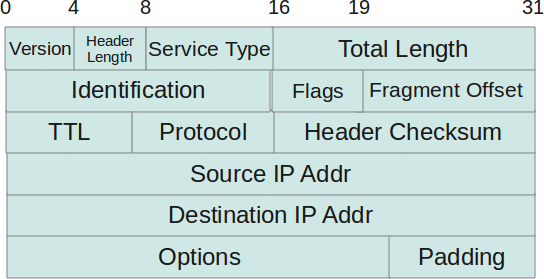
\includegraphics[width=10cm]{22.png}\\
	\\Annahme: der Header umfasst nur 20 Byte (keine zusätzlichen Header-Felder in Verwendung).
	$MTU\,=\,1500\,byte$
	In jedem Paket können also \\
	$1500\,byte\,-\,20\,byte\,=\,1480\,byte$ gesendet werden.\\
	Wir benötigen also $ceiling(2980\,\,byte/1480\,byte)\,=\,3$ Fragmente \\
	\\Paket 1: ID:a, total\_length=1500, MF=1, Offset=0 \\
	Paket 2: ID:a, total\_length=1500, MF=1, Offset=185 \\
	Paket 3: ID:a, total\_length=60,   MF=0, Offset=370 \\
	Original Paket: ID=a, total\_length:3000, MF=0, Offset=0\\
	
	Das original-Paket wird in 3 Fragmente aufgeteilt. Jedes hat einen Offset, der in 8 byte Schritten angegeben wird. Die Fragmente enthalten außerdem die ID des originalen Pakets, um sie als zusammengehörig erkennen zu können. Weiters wird die gesamte Länge sowohl beim originalen Paket, wie auch bei allen Fragmenten angegeben. Bei den ersten beiden Fragmenten wird zusätzlich die M-Flag gesetzt, die angibt, dass noch weitere Fragmente zu erwarten sind. Beim original Paket ist keine M-Flag gesetzt und der Offset ist 0.
		
	
\end{document}